\subsection{Ejercicio 16}
\graphicspath{ {img/16} }


Antes de realizar el proceso con la VPN de la UDC, comprobamos nuestras direcciones IP privada y pública junto con la calidad de la conexión de la misma manera que en el ejercicio anterior. Mostraremos las características en las figuras \ref{fig:IPs-preUDC} y \ref{fig:Calidad-Conexión-preUDC}.

\begin{figure}[H]
    \centering
    \begin{subfigure}{.5\textwidth}
        \centering
        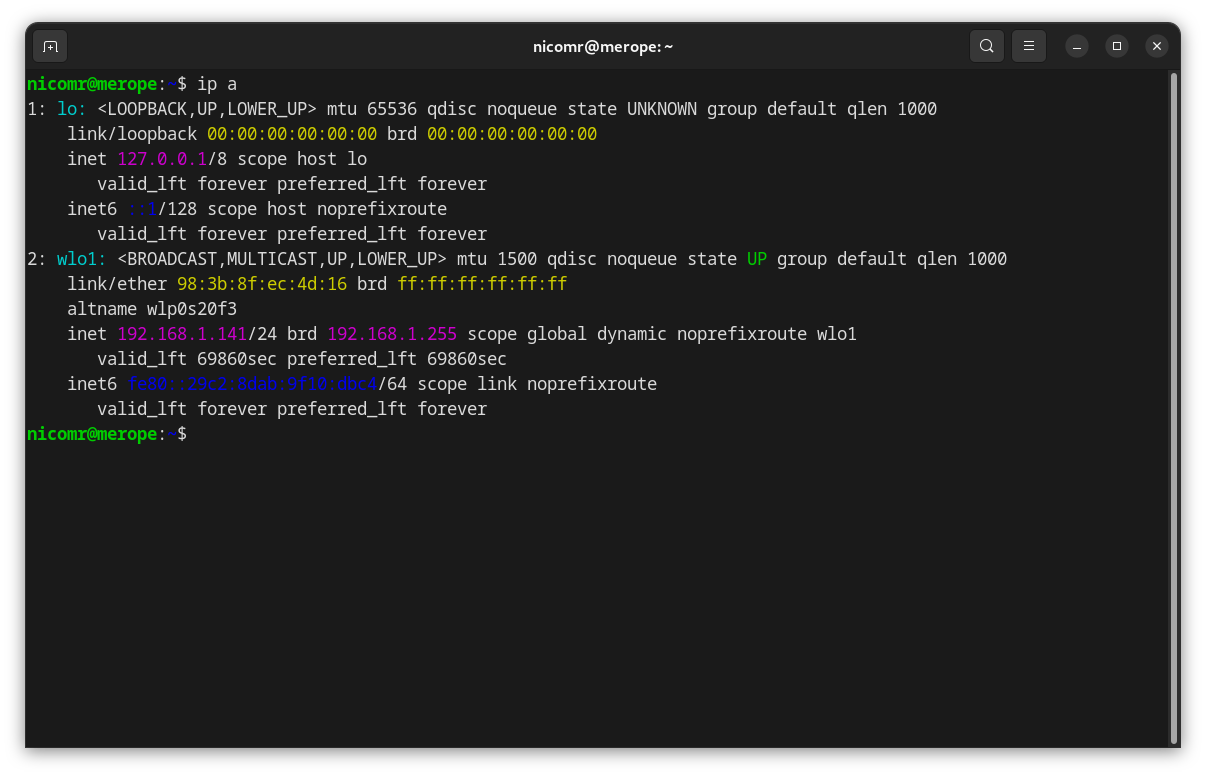
\includegraphics[width=\linewidth]{IP-Privada-UDC.png}
        \caption{Dirección IP Privada}
    \end{subfigure}%
    \begin{subfigure}{.5\textwidth}
        \centering
        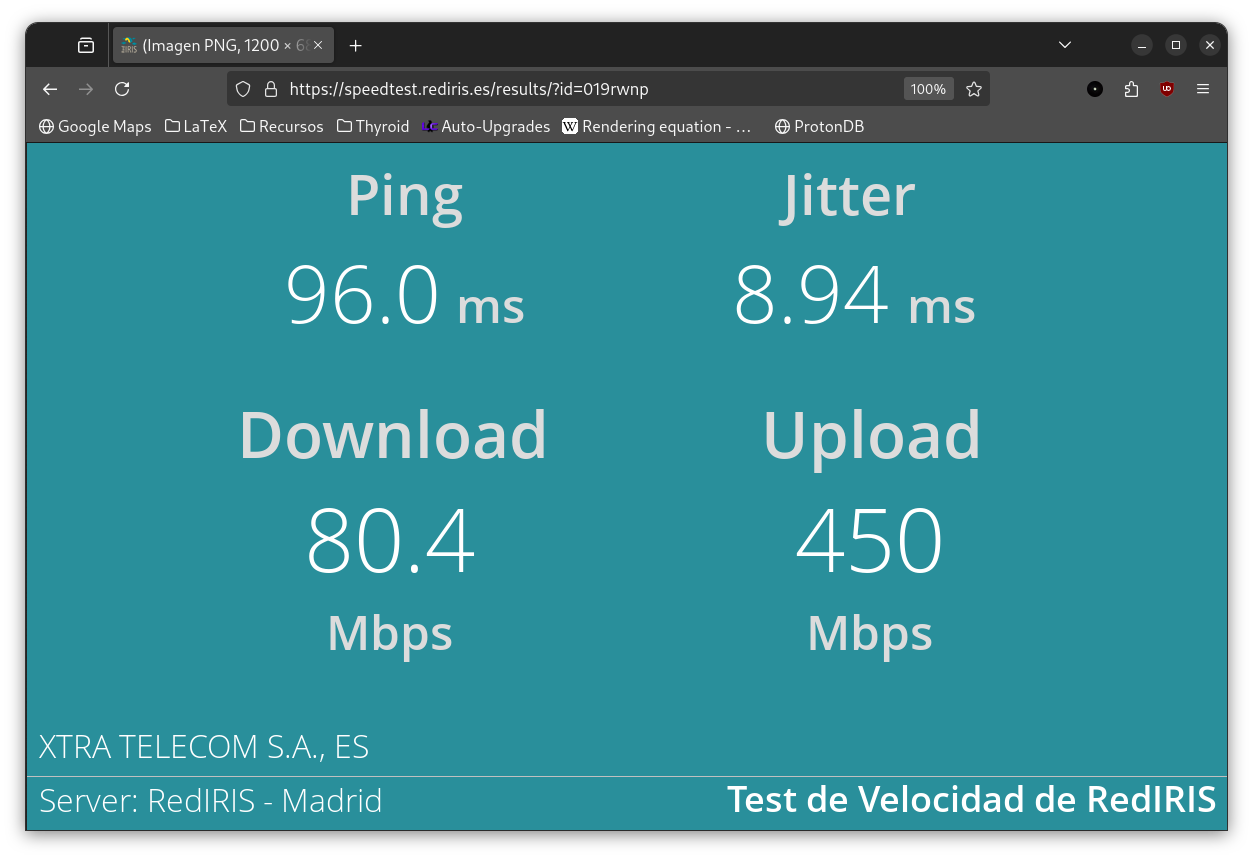
\includegraphics[width=\linewidth]{IP-Publica-UDC.png}
        \caption{Dirección IP Pública}
    \end{subfigure}
    \caption{Direcciones IP antes de utilizar la VPN de la UDC}
    \label{fig:IPs-preUDC}
\end{figure}

\begin{figure}[H]
    \centering
    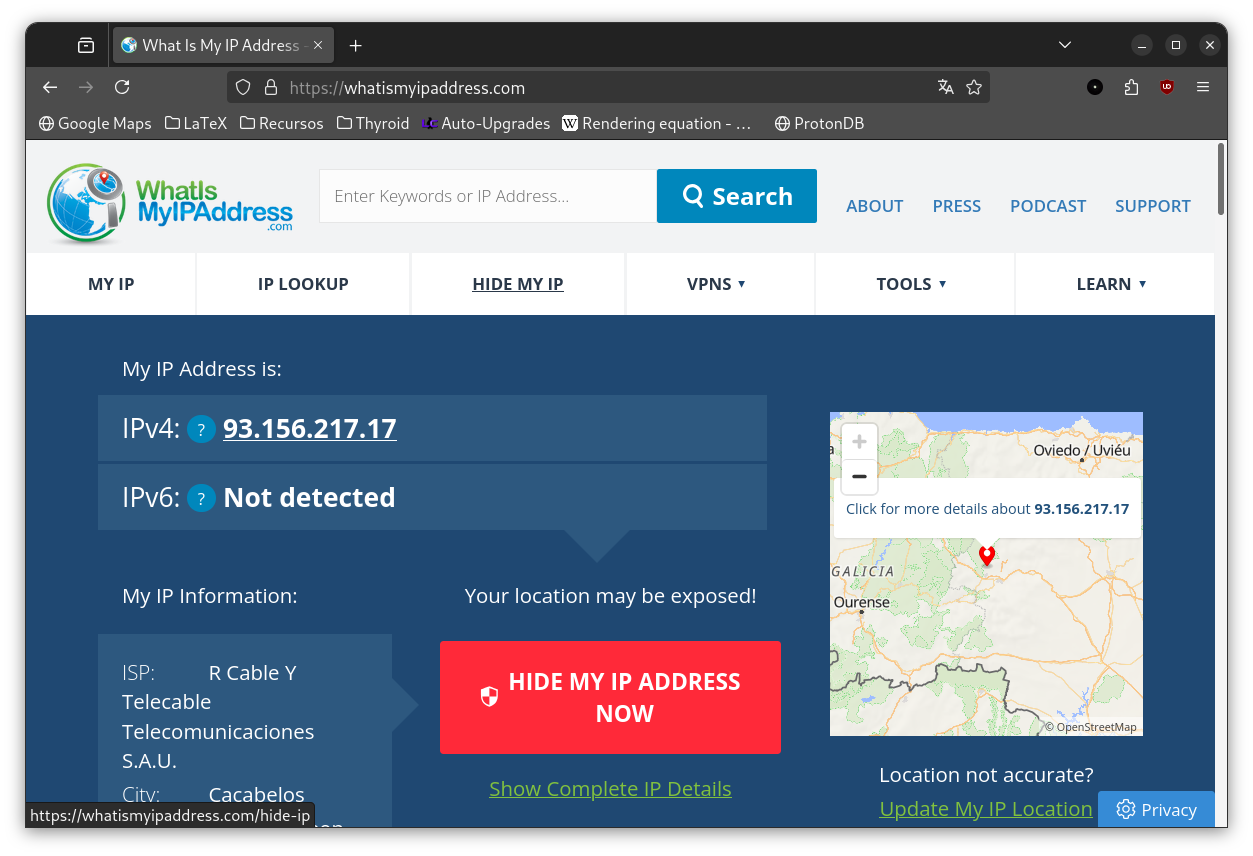
\includegraphics[width=\linewidth]{CalidadConexion-UDC.png}
    \caption{Calidad de la conexión antes de utilizar la VPN de la UDC}
    \label{fig:Calidad-Conexión-preUDC}
\end{figure}


Para utilizar la VPN de la UDC primero debemos instalarla y configurarla en el enlace \href{https://axudatic.udc.gal/pages/viewpage.action?pageId=45813771}{\texttt{VPN-UDC}}, dentro del apartado \texttt{`Instalación e configuración'}.

Con la VPN instalada,
